%! Author = lazza
%! Date = 03/05/2022

\section{Exception handling}\label{sec:exception-handling}
The \textbf{interrupt} is an exception, cause by an internal or external event which alters the normal flow of control: this
must be processed by another program, the interrupt handler.

\subsection{Causes}\label{subsec:causes}
Asynchronous, external events:
\begin{itemize}[noitemsep]
    \item I/O device service-request
    \item timer expiration
    \item power disruptions, hw failure
\end{itemize}

Synchronous internal event:
\begin{itemize}[noitemsep]
    \item undefined opcode, privileged instruction
    \item arithmetic overflow, FPU exception
    \item misaligned memory access
    \item virtual memory exceptions: page faults, TLB miss, protection violations
    \item traps: system calls, e.g., jumps into kernel
\end{itemize}

\subsection{Exception classes}\label{subsec:exception-classes}
\begin{description}
    \item[Sync vs Async] async caused by devices external to the CPU and memory and can be handled easily
    \item[User request vs coerced] user requested are predictable: treated as exceptions because they use the same
    mechanism that are used to save and restore the state handled after the instruction has completed.
    Coerced are caused by some HW event not under control of the program.
    \item[User maskable vs user nonmaskable] The mask simply controls whether the hardware responds to the
    exception or not.
    \item[Within vs between instructions] Exceptions that occur within instructions are usually
    synchronous since the instruction triggers the exception.
    The instruction must be stopped and restarted.\\
    Asynchronous that occur between instructions arise from
    catastrophic situations and cause program termination.
    \item[Resume vs terminate] Terminating event: program’s execution always stops after the
    interrupt.
    Resuming event: program’s execution continues after the
    interrupt.
\end{description}

\begin{figure}[h]
    \centering
    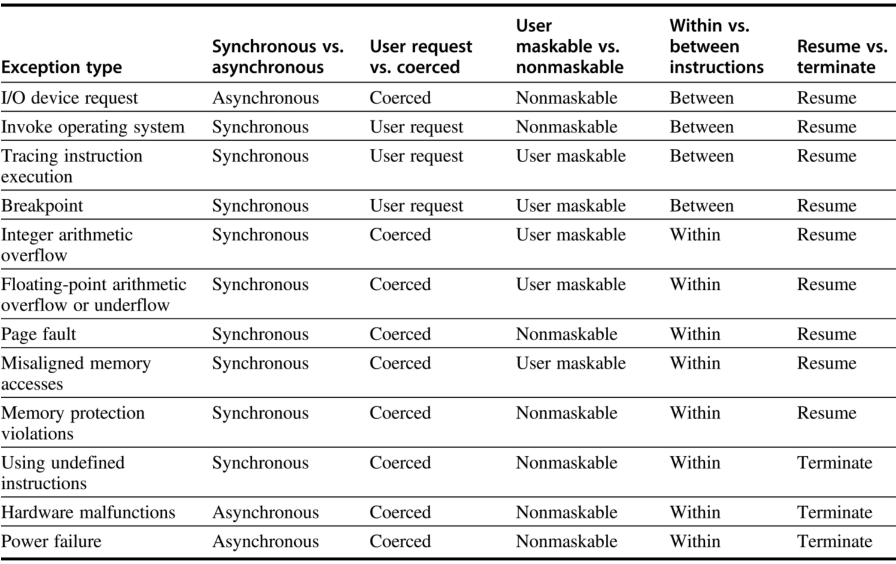
\includegraphics[scale = 0.25]{images/classes-of-exception}
    \caption{Exception classes}
    \label{fig:exception-classes}
\end{figure}

\subsection{Interrupt handler}\label{subsec:interrupt-handler}
When an I/O device requests attention, by asserting one of the prioritized interrupt request lines, the CPU, if
possible, invokes the interrupt handler.
When the processor decides to process the interrupt:
\begin{itemize}[noitemsep]
    \item It stops the current program at instruction I, completing all the previous instructions (precise interrupt)
    \item It saves the PC of instruction I in a special register (EPC)
    \item It disables interrupts and transfers control to a designated interrupt handler running in the kernel mode.
\end{itemize}
The cpu we have two modes: user-mode and kernel-mode.

The \textbf{interrupt handler} saves PC before allowing nested interrupts.
Needs to read a \textit{status register} that indicates the cause of the interrupt.
Uses a special indirect jump instruction RFE
(Return-From-Exception) which:
\begin{itemize}[noitemsep]
    \item enables interrupts
    \item restores the processor to the user mode
    \item restores hardware status and control state
\end{itemize}

\subsection{Synchronous interrupts}\label{subsec:synchronous-interrupts}
A sync interrupt is caused by a particular instruction.
In general, the instrucion cannot be completed and needs to restarted after the exception has been handled.
In case of a system call trap, the instruction is considered to have been completed.

\subsection{Precise Interrupts/Exceptions}\label{subsec:precise-interrupts/exceptions}
An interrupt or exception is considered precise if there is a single
instruction (or interrupt point) for which all instructions, before that
instruction, have committed their state and no following instructions
including the interrupting instruction have modified any state.
This means, effectively, that you can restart execution at the interrupt point.
\begin{figure}[h]
    \centering
    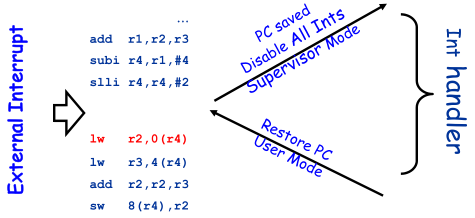
\includegraphics[scale = 0.4]{images/precise-interrupt}
    \caption{Precise interrupt}
    \label{fig:precise-interrupt}
\end{figure}


